\documentclass{standalone}
\usepackage{tikz}
\begin{document}
    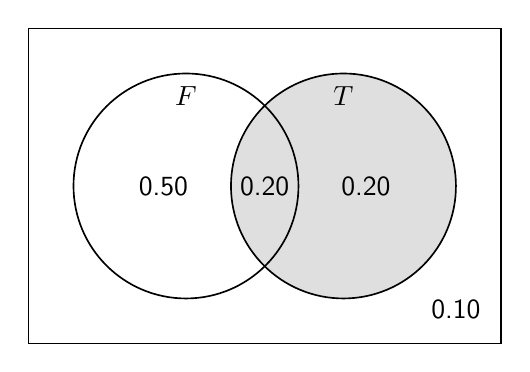
\begin{tikzpicture}[scale=2/7,font=\sffamily]

        \draw[semithick] (0,0) rectangle (21,14);

        % Sets: Path is fill, draw is bddry
        \path[fill=white] (7,7) circle (5);
        \path[fill=gray!25] (14,7) circle (5);
        \draw[semithick] (7,7) circle (5);
        \draw[semithick] (14,7) circle (5);

        % Set names
        \node at (7,11) {$F$};
        \node at (14,11) {$T$};

        % Numbers in each region
        \node at (6,7) {0.50};  % Only in X
        \node at (10.5,7) {0.20};    % Intersection
        \node at (15,7) {0.20};   % Only in Y
        \node at (19,1.5) {0.10};   % Complement of union
    \end{tikzpicture}
\end{document}